\appendix

\section{Description of datasets}

Most of the VQA datasets contain ambiguities and have strong linguistic biases that allow a model to learn answering strategies that exploit those biases, without reasoning about the visual input ~\cite{Santoro2017ASN}
The CLEVR dataset ~\cite{johnson2017clevr}  was developed to address those issues and come back to the core challenge of visual QA which is reasoning  \href{url}{https://arxiv.org/pdf/1612.06890.pdf}.\\
CLEVR contains images of 3D-rendered objects, such as spheres and cylinders. Each image is associated with a number of questions that fall into different categories. For example, query attribute questions may ask “What is the color of the sphere?”, while compare attribute questions may ask "Is the cube the same material as the cylinder? ”.
The dataset consist of:
\begin{itemize}
\item 	A training set of 70k images and 700k questions
\item	A test  set of 15k images and 150k questions about objects
\item	A validation set of 15k images and 150k 
\item	Answers, scene graphs and functional programs for all train and val images and questions

\end{itemize}

The dataset features unbiased, highly compositional questions that require an array of challenging reasoning skills, such as transitive and logical relations, counting and comparisons, without allowing any shortcuts around such reasoning ~\cite{hudson2018compositional}.

To test how well models learn compositional concepts that generalize, CLEVR-CoGenT was introduced . This dataset is synthesized in the same way as CLEVR but contains two conditions. As shown in Table 3 in Condition A, all cubes are gray, blue, brown, or yellow and all cylinders are red, green, purple, or cyan; in Condition B, cubes and cylinders swap color palettes.
Both conditions contain spheres of all colors. CLEVR-CoGenT thus indicates how a model answers CLEVR questions: by memorizing combinations of traits or by learning disentangled or general representations ~\cite{perez2017film}

This dataset consists of:
\begin{itemize}
\item	A training set of 70,000 images and 699,960 questions in Condition A
\item	A validation set of 15,000 images and 150,000 questions in Condition A
\item	A validation set of 15,000 images and 149,991 questions in Condition B
\item	A test set of 15,000 images and 149,980 questions in Condition B
\item	A test set of 15,000 images and 149,992 questions in Condition B
\item	Answers, scene graphs and functional programs for all train and val images and questions
\end{itemize}

\begin{table}
	\centering
	\begin{tabular}{ccccCcCc}
		\toprule
		Dataset        & Cubes              & Cylinders &  Spheres         \\
		\midrule
		CLEVR   &  any color &  any color        &    any color    \\
		%\midrule
		CLEVR CoGenT A & gray / blue / brown / yellow  & red / green / purple / cyan       &    any color  \\
		CLEVR CoGenT B  & red / green / purple / cyan &   gray / blue / brown / yellow       &      any color  \\
		\bottomrule
	\end{tabular}
	\caption{Comparison of the different colors/shapes combinations between CLEVR, CLEVR CoGenT-A and CLEVR CoGenT-B  }
	\label{tab:parameters}
\end{table}

\section{Full MAC and S-MAC comparison}

We think that in the main paper we should leave:
\begin{itemize}
\item first row - MAC - train on CLEVR, test on CLEVR 
\item all rows regaring S-MAC
\end{itemize}

When we will fill the whole table we will copy the results in here.

\section{Illustration of failures of MAC on CLEVR}
Following the evaluation of MAC on CoGenT-B, we built a tool which helped us visualizing the attention of the model over the question words and the image, and thus provide insight on some cases of failure.

\begin{figure}[]
	\centering
	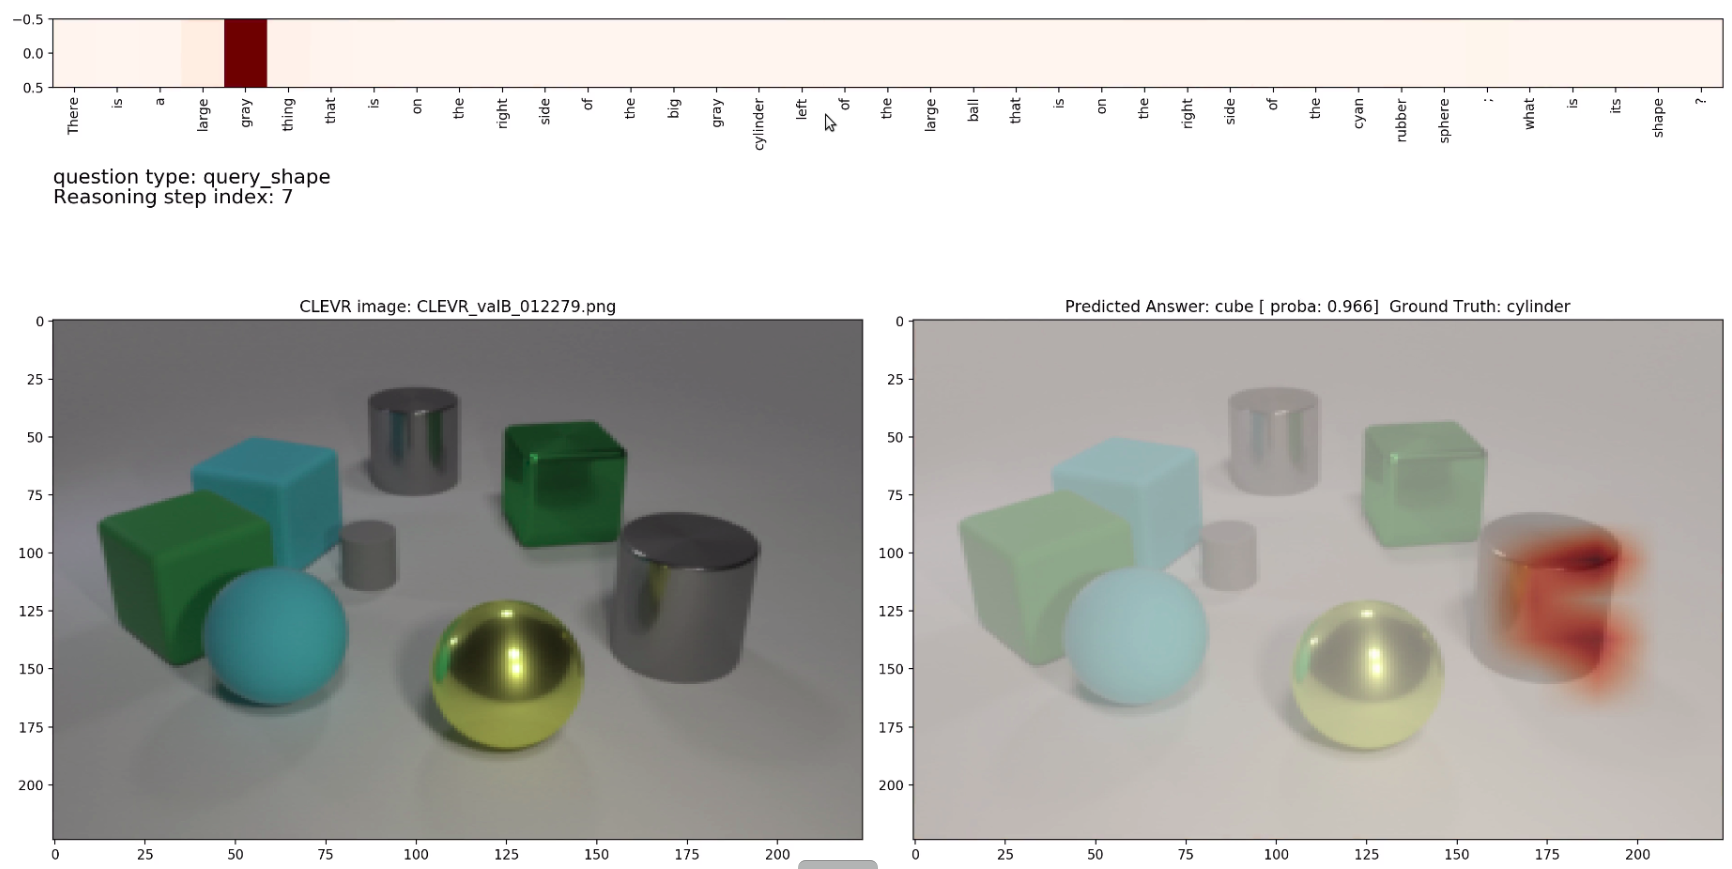
\includegraphics[width=\textwidth]{img/fail_mac_cogent_b_shape.png}
	\caption{The question reads as: \textit{There is a large gray thing that is on the right side of the big gray cylinder left of the large ball that is on the right side if the cyan rubber sphere; what is its shape?}}
	\label{fig:fail_mac_shape}
\end{figure}

\begin{figure}[]
	\centering
	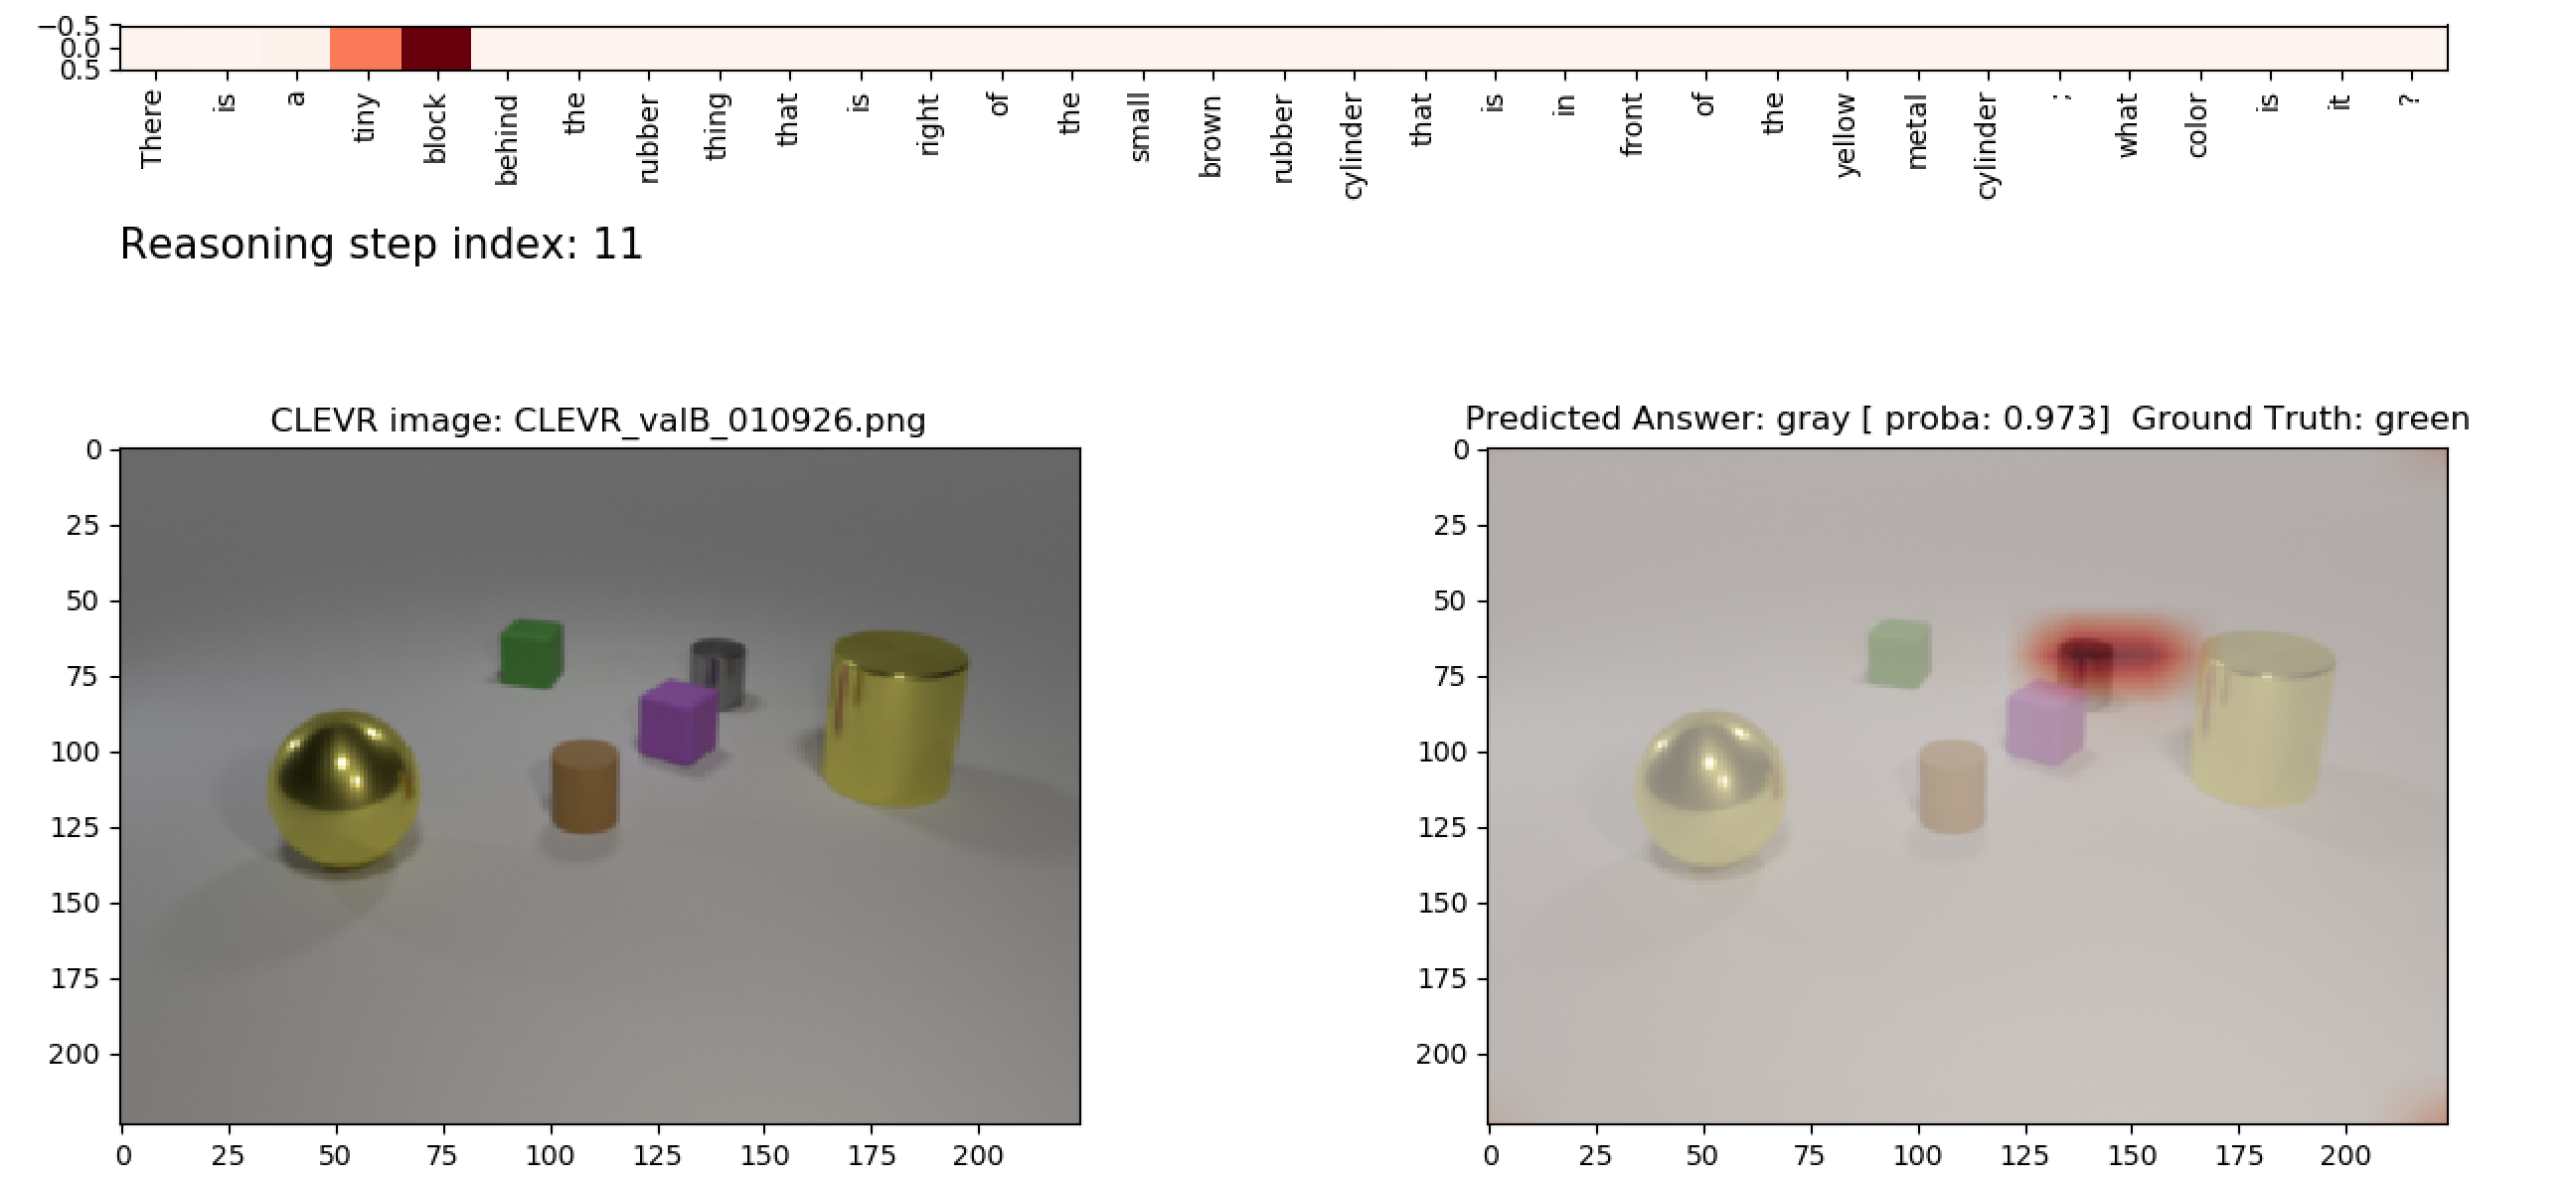
\includegraphics[width=\textwidth]{img/fail_mac_cogent_b_color.png}
	\caption{The question reads as: \textit{There is a tiny block behind the rubber thing that is right if the small brown rubber cylinder that is in front of the yellow metal cylinder; what color is it?}}
	\label{fig:fail_mac_color}
\end{figure}

\fig{fig:fail_mac_shape} presents a question where the model is asked about the shape of the leftmost gray cylinder. The model correctly finds it, as we can see from its visual attention map, and appears to refer to it using its color (\textit{gray}), as we can see from the attention of the question words. Yet, it defaults to predicting the shape as \textit{cube}, because it never saw gray cylinders during training, but instead saw gray cubes.

\fig{fig:fail_mac_color} presents a similar case, where the model is questioned about the color of the green cube at the back. MAC misses that object, and instead focuses on the nearby gray cylinder. We can hypothesize that MAC missed the green cube as it did not see this combination during training, and thus default to a combination that it knows.

Those examples indicate that MAC did not correctly separate the concept of shape from the concept of color, but have a better understanding of the colors (as it found the object of interest in \fig{fig:fail_mac_shape} by its color). This could come from that fact that the shape \textit{sphere} is associated with all possible colors in the dataset. 